\begin{ex}
Um sistema cartesiano foi associado a uma região plana de modo que o eixo Ox está orientado de oeste para leste, o eixo Oy está orientado de sul para norte, e a unidade adotada nos eixos é o quilometro.
   \begin{enumerate}[(a)]
   \item Pedro deve caminhar do ponto O(0,0) até A(5,4) deslocando-se 1 quilômetro de cada vez para o norte ou para leste.
   Um caminho possível nessas condições é:
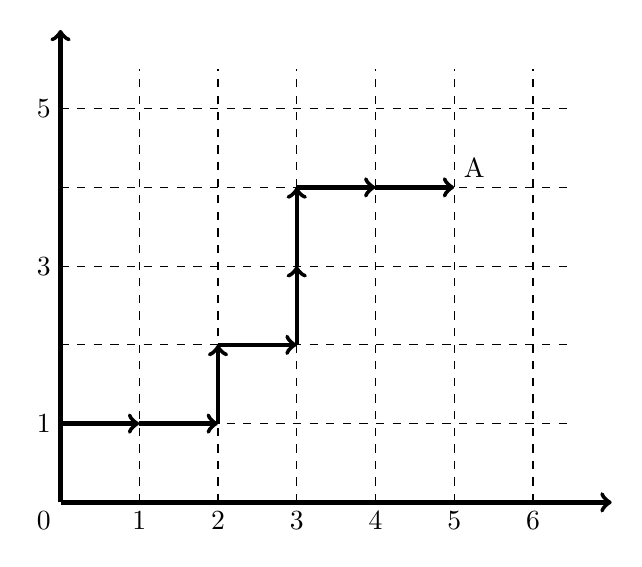
\begin{tikzpicture}
\draw [ultra thick] [- >] (0,0)--(7,0);
\draw [ultra thick] [- >] (0,0)--(0,6);
\draw [dashed] (0,1)--(6.5,1);   \draw [dashed] (0,2)--(6.5,2);
\draw [dashed] (0,3)--(6.5,3);   \draw [dashed] (0,4)--(6.5,4);
\draw [dashed] (0,5)--(6.5,5);   \draw [dashed] (1,0)--(1,5.5);
\draw [dashed] (2,0)--(2,5.5);   \draw [dashed] (3,0)--(3,5.5);
\draw [dashed] (4,0)--(4,5.5);   \draw [dashed] (5,0)--(5,5.5);
\draw [dashed] (6,0)--(6,5.5);   \draw [ultra thick] [->] (0,1)--(1,1);
\draw [ultra thick] [->] (1,1)--(2,1); \draw [ultra thick] [->] (2,1)--(2,2);
\draw [ultra thick] [->] (2,2)--(3,2); \draw [ultra thick] [->] (3,2)--(3,3);
\draw [ultra thick] [->] (3,3)--(3,4); \draw [ultra thick] [->] (3,4)--(4,4);
\draw [ultra thick] [->] (4,4)--(5,4); \draw node [above right] at (5,4) {A};
\draw node [left] at (0,1) {1}; \draw node [left] at (0,3) {3};
\draw node [left] at (0,5) {5}; \draw node [below left] at (0,0) {0};   
\draw node [below] at (1,0) {1};\draw node [below] at (2,0) {2};
\draw node [below] at (3,0) {3};\draw node [below] at (4,0) {4};
\draw node [below] at (5,0) {5};\draw node [below] at (6,0) {6};
\end{tikzpicture}

   Quantos caminhos diferentes Pedro pode percorrer de 0 até A?
   \item Luís deve caminhar de O(0,0) até B(6,5), passando por C(4,3), deslocando-se 1 quilômetro de cada vez para o norte ou para leste.
   Quantos caminhos diferentes Luís pode percorrer?
   \end{enumerate}
    \begin{sol}
      \phantom{A}
       \begin{enumerate} [(a)]
           \item $\frac{9!}{4!\cdot5!}=126$
           \item $\frac{7!}{3!\cdot4!}\cdot\frac{4!}{2!\cdot2!}=210$
       \end{enumerate}
    \end{sol}
\end{ex}